\chapter{基于软件定义网络和边缘计算的异构车联网架构研究}
本章将针对基于软件定义网络和边缘计算的异构车联网架构进行研究。
本章内容安排如下:\ref{section 2-1} 节是本章的引言,介绍车联网服务架构研究现状和目前研究的不足以及本章的主要贡献。
\ref{section 2-2} 节阐述本章的异构车联网架构设计。
\ref{section 2-3} 节介绍异构车联网中面临的挑战与机遇。
\ref{section 2-4} 节通过两个实例研究分析了不同架构下ITS典型应用的性能并给出相应启示。
\ref{section 2-5} 节总结本章的研究工作。

\section{引言}\label{section 2-1}
随着无线通信、传感、计算和控制等技术的蓬勃发展,车联网正逐步发展成为实现智能网联汽车、自动驾驶和智能交通系统等尖端技术应用的范式。
基于蜂窝的V2X通信、大数据分析和人工智能的发展将进一步推动这一趋势,预示着汽车行业的下一场革命即将到来。
回顾过去十余年手机的发展历程,可以看到手机已经从传统的通话和信息传递工具转变为具有社交、导航、多媒体娱乐等诸多功能的智能设备。
同样,在不久的将来,汽车也将发生类似的趋势。
汽车不再仅是简单的运输工具,而且将朝着智能化、网联化、协同化方向演进,并成为支撑各种智能交通系统应用的关键。
因此,当前亟需为未来的车联网开发新的范例。
本章致力于提出一种新颖的异构车联网系统架构,通过综合软件定义网络和边缘计算的范式特征,最大化端边云的协同效应,提供实时、可靠和大规模的车联网信息服务。

为了改造和革新传统的网络架构,研究人员提出了软件定义网络\cite{wang2020ji},其实现逻辑上的集中控制与网络功能快速迭代。
目前,SDN 在云计算系统中的控制和管理已经显示出了巨大的优势\cite{jain2013network}。
其核心思想是通过解耦网络中的控制平面和数据平面来简化管理,加速网络系统的演进。
在控制平面,网络中的控制功能集中于 SDN 控制器,并通过基于软件的方式实时修改和更新网络传输规则。
在数据平面,网络节点(如交换机)将根据 SDN 控制器的决策转发数据包。
然而,车联网的快速发展给传统的车联网架构带来了诸多挑战。
例如,传统的网络架构中,网络控制和数据转发功能耦合在一起,难以满足车联网中时变网络需求,并满足车联网实时性、可靠性和安全性等性能需求。
而基于SDN的网络架构,可以将网络控制和数据转发的功能解耦,实现网络资源的灵活配置和优化。
具体地,SDN可以把车联网中的控制器放在云端,实现对车联网中所有的流量进行集中控制。
此外,SDN的虚拟化技术可以将车联网中的物理资源虚拟化,使得网络资源管理更为高效和灵活。
通过SDN技术,车联网可以实现更加精细化的管理和调度,提高网络的可靠性和性能,为智能交通系统应用提供更好的支持。
考虑到车联网的特点,如动态网络拓扑、车辆的高移动性和异质通信接口,亟需一个基于 SDN 的框架来抽象资源,并在该系统中实现最佳服务调度。

另一方面,边缘计算是一种新兴的网络模式,其能够在物联网时代为数十亿联网设备提供高可靠性和低延迟的信息服务 \cite{shi2016edge}。
边缘计算通过将计算、网络、存储资源从云端卸载到终端用户附近,从而有效地缩短数据传输和响应时间,提高服务的可靠性和响应速度。
与传统的基于云的服务不同,边缘计算专注于支持高密度的设备连接和网络边缘的密集计算。
毋庸置疑,车联网作为物联网中最具代表性的应用场景之一,有望从基于边缘的服务发展中获得巨大的收益。
车联网不仅代表着车辆之间的连接,更重要的是,它还代表着行人、道路、基础设施等之间的协作。
通过边缘计算技术,车联网能够实现实时数据采集、处理和传输,使车辆之间的协作更加高效和精确。
同时,边缘计算还可以通过在车辆和设施之间构建更加紧密的联系,实现更加智能的交通控制,从而提高交通安全和效率。
值得注意的是,5G 技术的成熟和现代汽车在计算、存储和通信能力方面的快速发展,正强力驱动着边缘计算与车联网的联合 \cite{li2021che}。
超可靠和低延迟的5G技术可以大幅提高数据传输和响应速度,进一步提升车联网的效率和可靠性。
而现代汽车的智能化趋势也为边缘计算的应用提供了更为广泛的可能性。
未来,随着边缘计算技术的不断发展,车联网有望实现更加高效、安全、智能的交通运行。

针对车联网中的服务架构,研究人员在研究基于 SDN 和边缘计算的范式方面付出了巨大努力。
自Liu等人 \cite{liu2016cooperative} 于 2016年首次将 SDN 应用于车联网中,大量研究人员围绕软件定义车联网展开了研究 \cite{dai2018cooperative, luo2018sdnmac, liu2018coding, zhang2022ac-sdvn, zhao2022elite, lin2023alps, ahmed2023deep}。
然而,现有大部分工作仅仅是在软件定义车联网架构的基础上从数据分发、路由缓存、数据安全等方面展开了研究,并没有对整体架构进行深入分析。
另一方面,越来越多的研究在车联网环境中考虑将边缘计算范式以提高系统实时性、可靠性、安全性\cite{liu2017a, lang2022cooperative, liu2021fog, dai2021edge, zhang2022digital, liu2020adaptive, liao2021learning, liu2023mobility, liu2023asynchronous}。
然而,上述研究并没有综合考虑异构车联网中最大化不同服务架构的协同效应,且绝大多数架构研究仍停留在理论分析层面,缺乏在实际场景中对架构优势进行验证。

基于以上分析,本章首先提出了车联网中信息服务的分层架构,包括应用层、控制层、虚拟层和数据层。
考虑到车联网的独特特征,包括车辆的高移动性、间歇性服务连接、动态网络拓扑和异构资源,本章结合了 SDN 和边缘计算范式以最大化不同范式的协同效应。
具体地,全面分析了车联网中控制和数据平面的分离、异构资源环境中的网络功能虚拟化、针对不同服务质量要求的服务的网络切片(Network Slicing, NS),以及基于边缘服务的计算、存储、控制和通信能力卸载。
此外,还讨论了该架构下产生的新挑战,并提出车联网的跨层协议栈,以指导未来的研究方向。
最后,搭建了两个原型系统,并在现实的车联网环境中实现了两个应用。
原型系统不仅验证了本章提出的异构车联网系统架构的可行性,而且为未来车联网的实际部署提供了参考。

\section{架构设计}\label{section 2-2}

本章提出了一个新颖的车联网分层架构,旨在增强信息服务的可扩展性和可靠性,提高应用管理的敏捷性和灵活性,并为下一代 ITS 的实现奠定坚实的基础。
如图 \ref{fig 2-1} 所示,该架构一共具有四层:应用层、控制层、虚拟层和数据层。
具体地,应用层是面向业务需求的最上层,包括各种 ITS 应用,例如安全认证、交通管理、数据管理等。
控制层是在应用层和虚拟层之间的一个逻辑层,负责管理和控制网络资源。
虚拟层是在底层硬件和控制层之间的一个中间层,用于虚拟化和管理网络、计算和存储资源。
数据层是位于底层,负责存储和处理车联网产生的各种数据,并提供对上层应用的数据支持。
分层结构使得不同层次的功能分离清晰,可分别进行优化和升级,同时也方便了系统的维护和管理。
简言之,分层架构的设计整合了SDN和边缘计算的范式,以最大限度地利用它们对车联网信息服务的协同效应。
其主要目标包括:a)在移动和动态网络环境中实现逻辑上的集中控制;b)在异构车联网环境中实现网络功能虚拟化,并为具有不同 QoS要求的服务实现网络切片;c)通过在基于云和边缘的服务之间进行协调,最大限度地利用车联网中的网络、计算、通信和存储资源。
车联网分层服务架构的详细设计介绍如下。

\begin{figure}[h] 
	\centering
	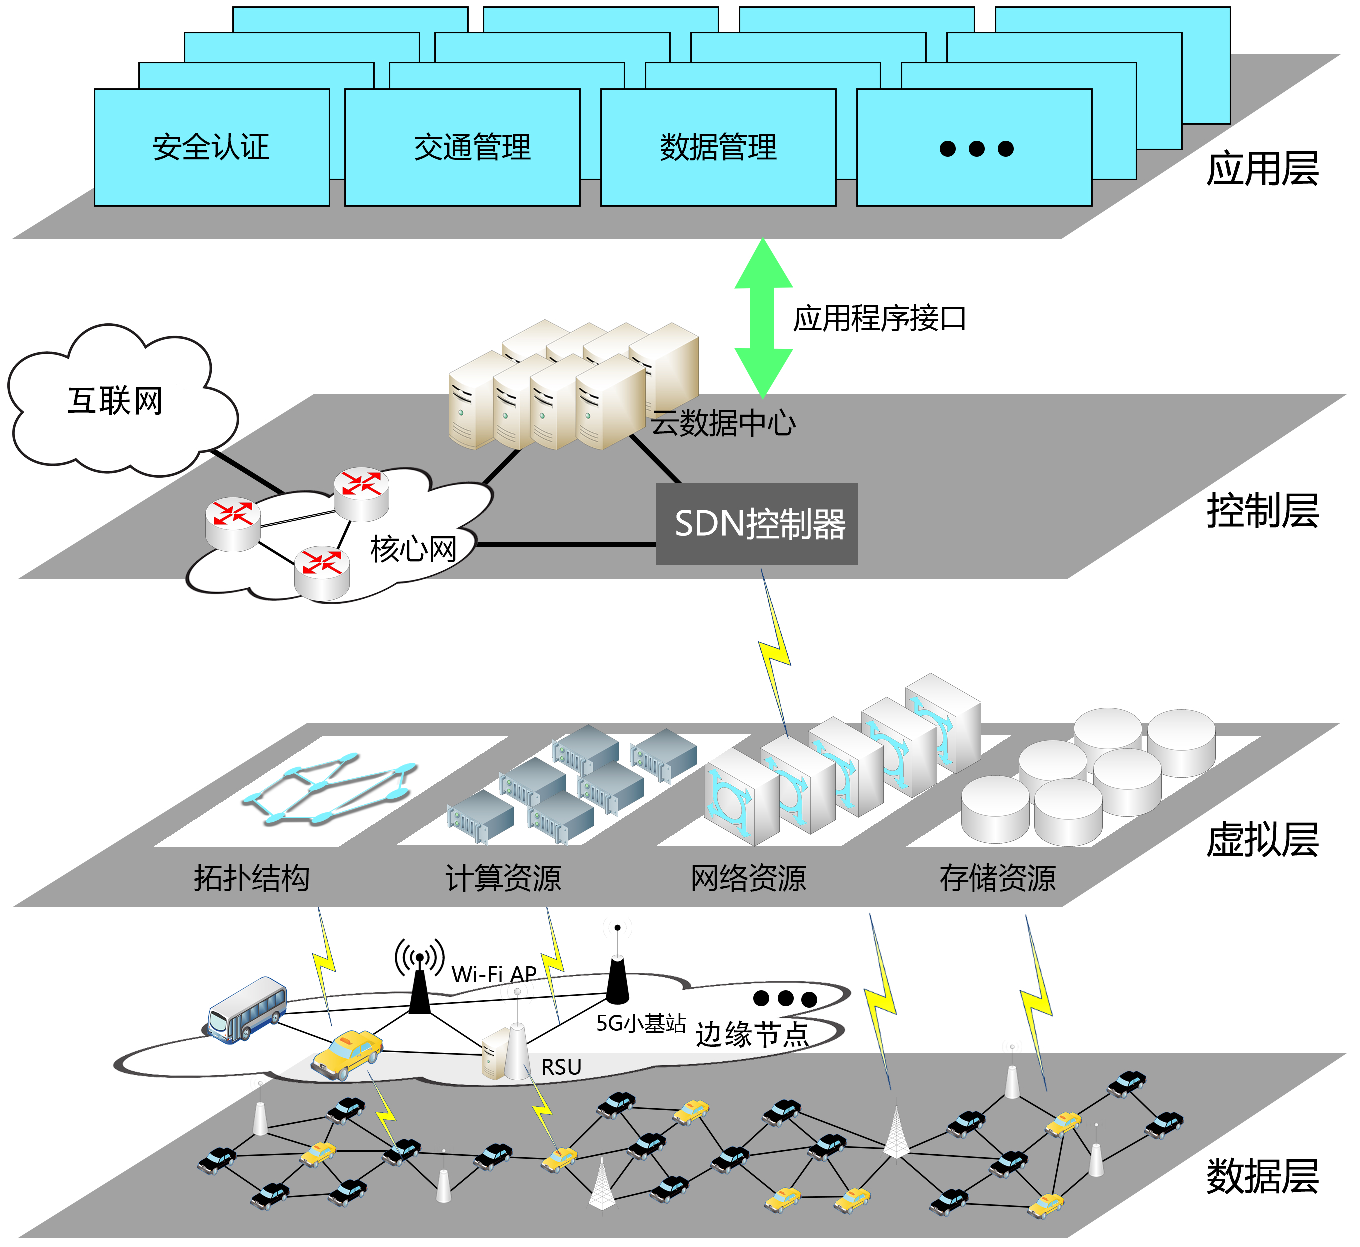
\includegraphics[width=1\columnwidth]{Fig2-1-hierarchical-architecture.pdf}
	\bicaption{异构车联网架构}{Hierarchical architecture for IoV}
	\label{fig 2-1}
\end{figure}

\subsection{基于软件定义网络的车联网集中控制}

在基于软件定义网络的车联网分层服务架构中,控制层中 SDN 控制器被部署在骨干网络中,并通过核心网络与云数据中心和互联网相连。
与传统SDN组件类似,该控制器通过北向接口与上层应用进行通信,例如安全认证、交通管理和数据管理等。
应用程序需要根据特定的需求使用相应的应用程序编程接口(Application Programming Interface, API)。
具体地,API接口可实现多维资源(例如计算、通信和存储资源)的分配、车辆行为控制、身份认证,以及访问控制等功能。
此外,SDN控制器通过南向接口与底层资源进行通信。
需要指出的是,控制器不需要直接管理异构的物理资源。
相反,通过直接使用虚拟层的资源抽象来获得虚拟资源的统一视图,从而促进SDN 控制器的业务调度。
虚拟层的资源抽象可以消除底层物理资源的复杂性,并为控制器提供更高的可靠性和性能。
因此,通过分层架构的设计,SDN 控制器不仅可以更好地管理车联网中的资源,而且可以提高车联网的可靠性和性能。
进一步,为了更好地支持车联网的高度动态性和异构性,控制层还提供了一些额外的功能。
例如,控制层还能够进行动态路由和流量调度,以应对车联网网络拓扑和负载的动态变化。
上述功能的整合使得SDN控制器可以更好地适应车联网的复杂环境,并提供高质量的信息服务。
值得注意的是,由于SDN控制器集中控制网络资源,因此可以提高网络的安全性和可靠性。
例如,控制器可以实现安全的访问控制,防止未经授权的用户访问网络资源。
此外,控制器还可以实现流量监测和QoS保障,从而提高网络的可靠性和服务质量。
上述服务实现的安全和可靠性的特性是车联网应用所必需的,因为上述应用涉及到交通安全和行车效率等关键问题,如果网络不稳定或者容易遭受攻击,则会对 ITS 应用的正常运行产生重大影响。

\subsection{车联网中网络功能虚拟化和网络切片}
虽然NFV和NS技术在5G网络中得到了广泛的研究 \cite{zhu2021wang},但是考虑到车联网中底层资源的高度异构和分布,以及上层ITS应用的高度动态和差异服务要求等特点,将其迁移到车联网中仍然面临着巨大挑战。
因此,本章提出了一个专门设计的虚拟层,它负责抽象车联网中的计算、网络和存储资源。
该虚拟层能够在物理基础设施之上提供更高层次的抽象,从而使应用程序能够更方便地访问底层资源。
然而,由于网络拓扑结构的快速变化、不同的无线通信接口的差异无线电覆盖范围,以及在数据层的节点之间不断产生、感知和共享的大量信息,构建并维持底层资源的准确逻辑视图是极具挑战的。
为了解决这个问题,本章考虑增加一个虚拟层,将部分数据节点(如公交车、出租车、5G小基站、RSU等)抽象为边缘节点。
边缘节点能够提供基于本地计算、通信和数据资源的服务,以及抽象和管理可用的本地资源。
一方面,边缘节点可以作为资源的管理者和协调者,负责管理和分配本地的计算、通信和存储资源,为上层应用提供优质的服务。
另一方面,边缘节点还可以作为数据的处理中心,对本地产生的数据进行处理和分析,从而降低数据的传输和处理延迟。
此外,由于边缘节点本身具有一定的智能,可以对诸如视频流、激光雷达点云数据等进行预处理和分析,从而进一步降低数据的传输和处理压力,提高系统的效率和可靠性。
通过上述方式,不仅降低了底层资源的动态性,也减少了上层资源虚拟化的工作量。
此外,这种分层架构有利于NFV和NS的垂直实施。
例如,给定一组具有各自QoS要求的应用,可以根据边缘的分布式调度或SDN控制器的集中式调度,以不同方式对虚拟资源进行协调。

\subsection{基于边缘计算的车联网分布式服务}

本章讨论的架构数据层由许多具有不同通信接口的节点组成,如 LTE 基站、RSU、Wi-Fi接入点(Access Point, AP)、5G 小基站和车辆。
除了不同无线通信接口接入能力外,这些节点还具备一定的计算和存储能力,其中部分节点被抽象为边缘节点,用于提供分布式服务。
相比较于以前在车联网中采用的独立的基于边缘的服务,本章设计的虚拟层顺利地弥合了SDN的逻辑集中控制和边缘层的分布式服务之间的差距。
在本架构中,移动和静态的数据节点都可以根据不同服务的调度动态地被分配为边缘节点(其中公交车、出租车等特种车辆可作为移动边缘节点)。
边缘节点不仅可以根据SDN控制器部署的规则执行操作,并且可以为本地服务实现某些智能,进一步提高服务质量和效率。
同时,边缘节点对底层资源进行一定的聚合和抽象,并向虚拟层实时更新状态,这反过来又有助于虚拟资源的管理。
因此,SDN 控制器可以更加方便地进行服务卸载和负载均衡的调度,从而进一步提高整个系统的性能。
除此之外,本架构还具有良好的灵活性和可扩展性。
由于边缘节点具有不同的通信接口和计算能力,因此它们可以根据实际需求进行灵活的配置和组合。
而且,随着新的节点不断加入系统,这个架构也可以随时进行扩展和升级,以适应未来的需求和挑战。

\section{架构挑战与机遇}\label{section 2-3}

本章节探讨了针对所提架构的新兴的挑战以及未来研究方向。
同时,本章提出了一个跨层协议栈,以指导未来车联网通信协议和服务算法的设计。

\subsection{控制层的全局知识获取}

为了实现逻辑上的集中控制,SDN控制器需要准确、及时地获取系统的全局知识,包括服务状态、资源状态、车辆状态等。
然而,在具有间歇性无线连接的高度动态车联网中,存在着诸多问题,例如传输延迟、数据包丢失和带宽竞争。
上述问题无法避免,并可能严重影响到控制层的全局知识获取和监控性能。
此外,在实践中,SDN 控制器通常是分布式部署在一个大型服务区域内。
因此,有效地整合来自多个控制器的信息,构建系统的全局逻辑视图,是至关重要的。
为了应对这些挑战,未来的研究可能会涉及到在控制层中引入新的模块,以弥补SDN控制器的失真视图和真实系统状态之间的差距。
此外,需要开发新的技术来高效地集成本地和分布式系统状态,构建全局系统知识的逻辑视图,实现分布式控制器之间的有效协调。
特别地,机器学习和人工智能技术可能会在优化控制层性能方面发挥至关重要的作用,通过动态适应车联网环境的变化,进一步推动基于SDN的车联网技术发展,为未来更高效、更可靠的车联网服务铺平道路。

\subsection{虚拟层的异构资源管理}

在实现网络切片的过程中,其中关键问题是如何统一一致地表征车联网中高度多样化和动态化的资源。
考虑到不同的通信接口可能会具有不同的无线电覆盖范围、传输速率和接入能力,不同通信资源的可用性和连接能力也可能随着网络拓扑结构的变化而动态变化。
此外,车联网中节点计算和存储资源的可用性也可能不断变化,因此可能导致虚拟化实体的服务协调难度增加。
例如,车辆或RSU等数据节点不断感知并产生新的数据,并进一步用于计算、传输和存储。
因此,如何为异质资源构建一个统一的、连贯的视图,并将其虚拟为切片实体是另一个值得未来努力的关键问题。

在车联网中,由于上层ITS应用的不断变化和不同的QoS要求,NFV 和 NS 需要能够协调虚拟化实体的服务。
然而,实现透明和自适应的服务以保证 QoS 要求是一项具有挑战性的任务。
例如,在虚拟化路由功能时,尽管数据平面和控制平面可以基于 SDN 进行解耦,但是仍然不能保证能在快速变化的车联网环境中为不断移动的车辆分配连续的资源。
因此,需要进一步研究基于边缘和云的服务之间的协作,以更好地管理和分配资源。
此外,在车联网中实现无缝和灵活的虚拟资源管理仍然具有挑战性。
尽管在数据层提出了基于边缘的分布式服务来帮助抽象化资源,但由于车联网中大规模分布和高度异质性的底层资源,如何在车联网中实现无缝和灵活的虚拟资源管理仍需要更多的研究和努力。
例如,在车联网中,不同的车辆和边缘设备具有不同的计算和存储资源,且它们的位置和连接性也会不断变化。
因此,需要考虑如何在车联网中动态地分配和管理虚拟资源,以满足不同车辆和设备的需求,并在保证QoS的同时提高系统的效率和灵活性。
为了解决这些挑战,需要继续深入研究和开发新的技术和算法,以实现更智能和自适应的虚拟资源管理。
例如,可以利用机器学习和人工智能技术来预测车辆和设备的资源需求,以更好地调度和管理虚拟资源。
此外,还可以探索更加分布式和去中心化的资源管理机制,以提高系统的可扩展性和鲁棒性。

\subsection{数据层中的大规模数据传输}

随着现代车联网中服务规模的快速增长和数据驱动型应用的蓬勃发展,现有的通信协议已经不能够有效地支持并行的 V2I/V2V 通信,特别是在高密度和高移动性的交通环境中。
因此,如何设计一种跨层的通信协议,以提高并发数据传输的资源利用率,成为了一个重要的研究方向。
目前,由于 C-V2X 仍处于演进阶段,IEEE 802.11p 已经成为了成熟的V2I/V2V通信标准,但是在大量基于 V2I/V2V 通信的数据传输在一定区域内同时进行时,由于其MAC层采用的载波监听多路访问(Carrier-Sense Multiple, CSMA)技术无法很好地处理并发数据传输,因此其带宽利用效率非常低。
因此,本章提出了一个跨层的通信协议设计,通过物理层的功率控制和MAC层的复用接入协议之间的共同设计,在传输范围、数据率和干扰之间取得平衡,从而提高数据吞吐量。

同时,在数据层更好地协调异质资源以实现大规模数据服务也至关重要。
然而,数据节点的存储、计算和通信能力方面存在异质性,这种差异可能会对系统性能产生负面影响。
另外,数据节点的移动性也增加了资源利用优化的挑战性。
为了解决这些问题,未来的研究可以利用不同类型车辆的移动模式和轨迹来优化系统性能。
例如,可以利用出租车的移动轨迹来动态地调整数据存储位置,以减少数据访问时的延迟。
此外,还可以利用公交车等大型交通工具的通信能力来提高数据传输速度,从而加速数据处理的过程。
然而,在实现这些方法时,需要解决数据安全和隐私保护等问题。
例如,需要确保数据存储在安全的位置,并采取必要的措施来保护数据的机密性和完整性。
同时,还需要考虑数据隐私保护的问题,例如,对用户个人信息的保护以及对敏感数据的访问控制等。

\subsection{跨层协议栈}

\begin{figure}[h] 
	\centering
	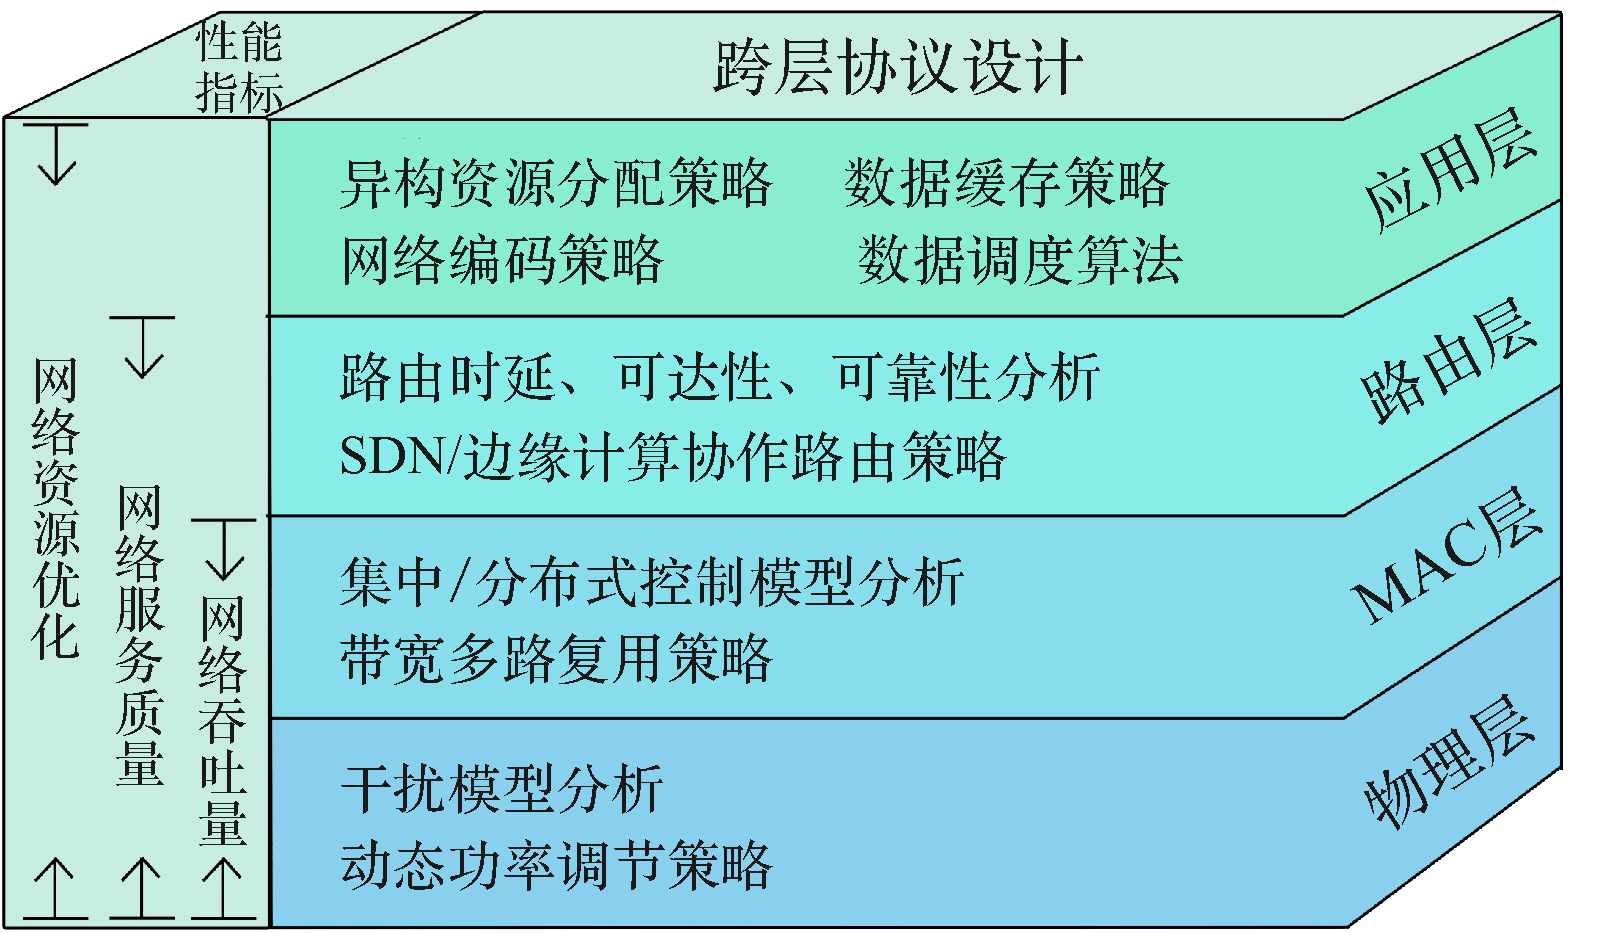
\includegraphics[width=1\columnwidth]{Fig2-2-protocol.pdf}
	\bicaption{跨层协议设计}{Overview of the cross-layer protocol stack}
	\label{fig 2-2}
\end{figure}


在下一代车联网中,为了实现高效的系统架构,需要协同设计通信协议和服务算法。
为此,本章提出了一种跨层协议栈如图 \ref{fig 2-2} 所示,其总体目标包括优化异构资源、提高系统性能,以及改善系统安全性。
跨层协议栈是一种将不同层级的协议集成到一个协议栈中的新型网络体系结构。
该设计可以在不同层级之间实现信息和资源的交互和协作,从而实现系统的整体优化。
在车联网中,由于网络拓扑结构和设备类型的异构性,跨层协议栈的设计尤为重要。
通过将应用层、路由层、MAC层和物理层的协议整合到一个跨层协议栈中,车联网可以更好地管理网络中的数据流和资源分配,从而提高系统的响应速度、可靠性和可扩展性。

然而,跨层协议栈需要解决一些开放性问题,例如如何设计信道模型和自适应功率控制策略,以实现合作的V2I/V2V通信;如何设计带宽复用机制和自适应资源分配策略,以实现并发数据传输;如何基于SDN设计面向QoS的数据路由协议,以实现高质量的服务;以及如何通过基于边缘的服务设计任务卸载和均衡的调度算法,以更好地管理和分配资源等。
具体地,合适的信道模型和功率控制策略是确保车辆间通信可靠性和信号质量的关键。
如何进行带宽复用和资源分配来保证多个数据流同时传输,同时避免网络拥塞和资源浪费也是需要考虑的问题。
如何设计面向QoS的数据路由协议来确保数据在网络中的流动性和服务质量是一个重要的研究方向。
如何通过基于边缘的服务设计任务卸载和平衡的调度算法来提高系统的性能是一个需要深入探讨的问题。

\section{案例研究}\label{section 2-4}

本章已经在真实的车联网环境中基于所提架构开发了两个原型系统,以验证其概念的可行性。
以上原型系统分别实现了“透视”和碰撞预警服务。
为了保证系统的稳定性和可靠性,采用云服务器作为SDN控制器,并连接到骨干网络,其通过基于 LTE 的通信进行集中式控制。
同时,Cohda Wireless MK5 RSU和OBU设备被用于通过DSRC进行V2V 和 V2I 通信。
在边缘层,一个RSU被安装在道路交叉口,并被连接到一个笔记本电脑,作为边缘节点以提供服务。
每辆车都配备了一个OBU以及一个带有LTE接口的平板电脑/笔记本电脑,车辆可以通过它与SDN控制器进行通信。
所有RSU和车辆的通信、计算和存储能力都可以抽象为虚拟资源。
为了满足应用层规定的服务要求,虚拟资源可以根据SDN控制器的某些调度算法进行自适应分配。

\subsection{“透视”服务}

\begin{figure}[h] 
	\centering
	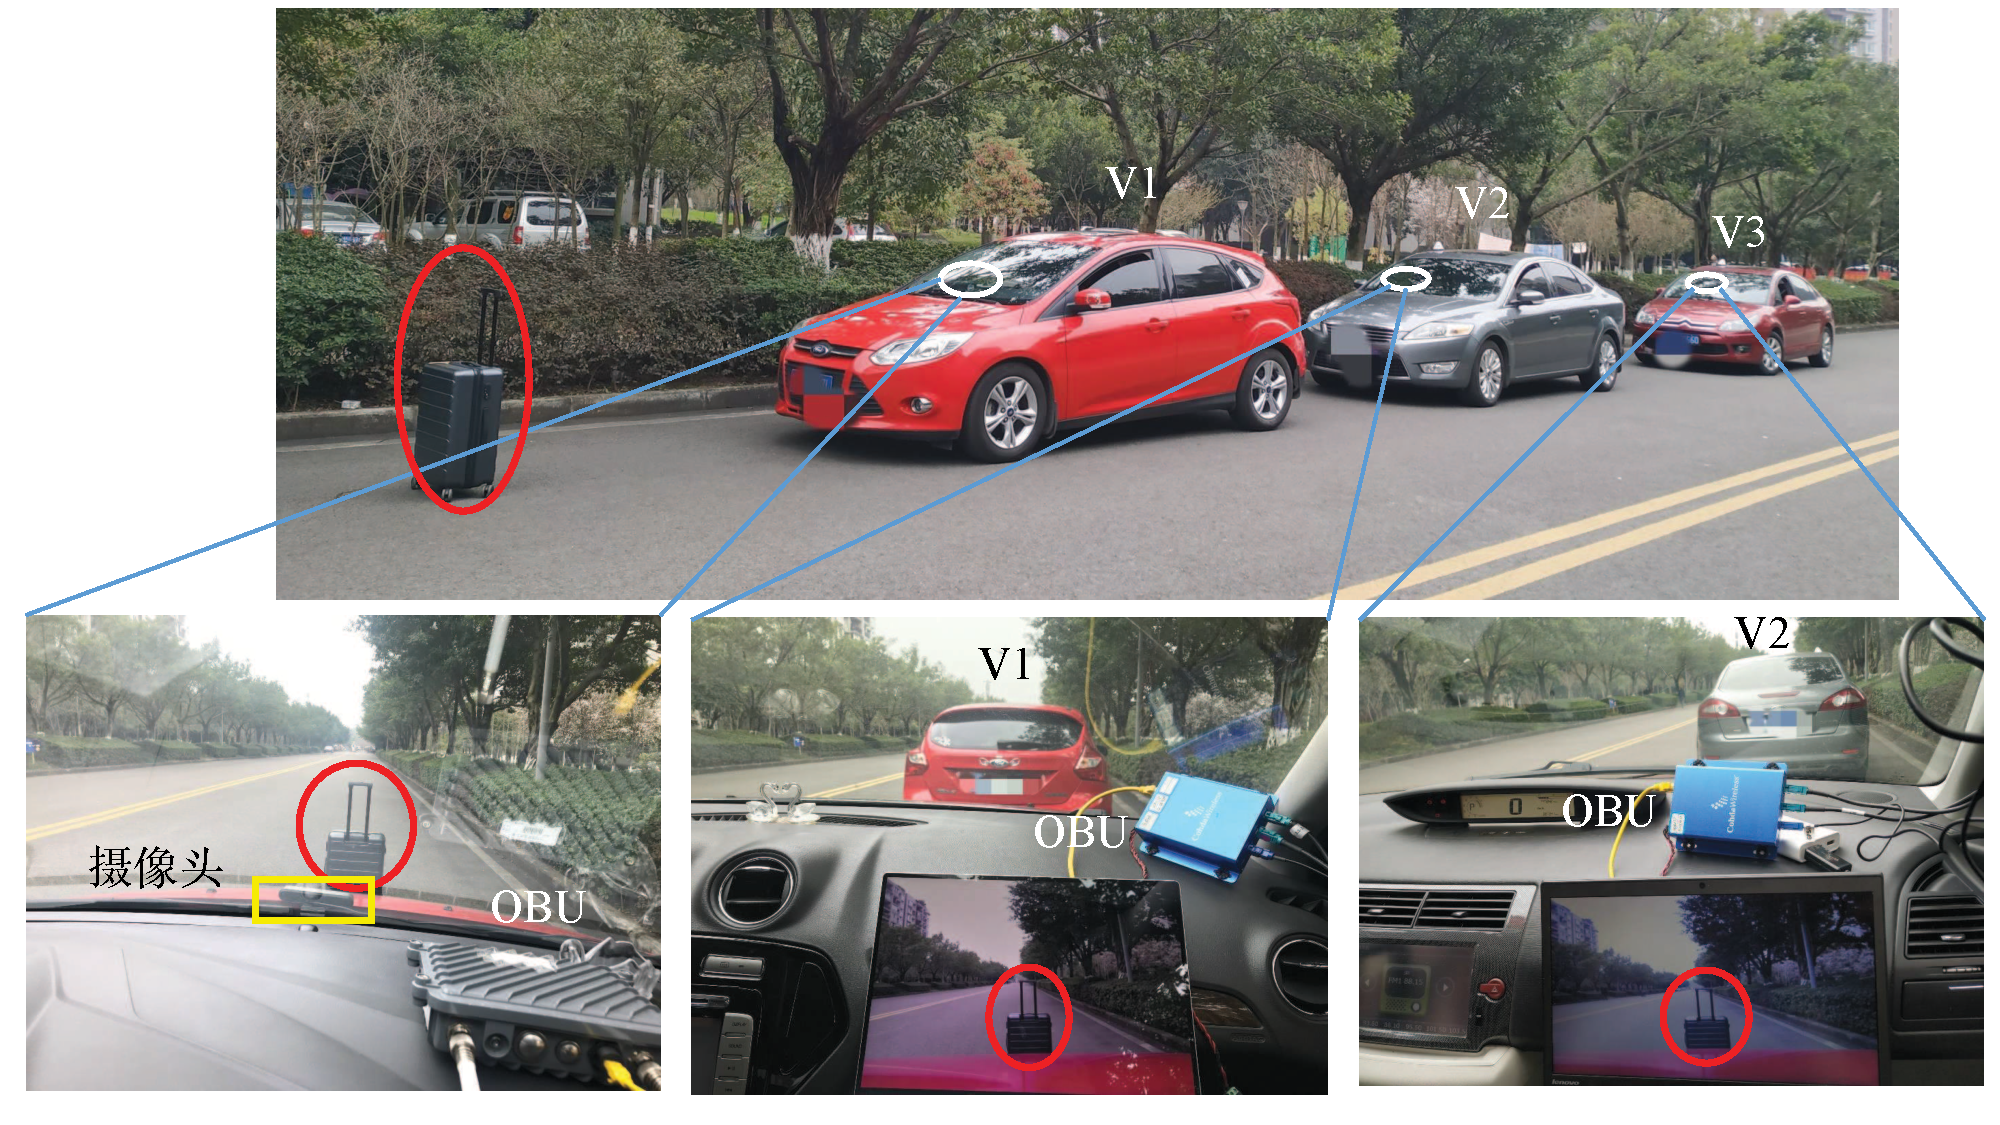
\includegraphics[width=1\columnwidth]{Fig2-3-case1.pdf}
	\bicaption{基于V2V通信的“透视”}{`See Through' via V2V communications}
	\label{fig 2-3}
\end{figure}

本章实现的“透视”服务如图\ref{fig 2-3}所示,该服务旨在将前方车辆的实时视图分享给后续车辆,从而提高行驶安全性。
在所提服务中,任何愿意分享视频摄像头拍摄的视图的车辆都可以通过基于LTE的通信在SDN控制器上注册其服务。
基于车辆拓扑结构和注册服务的全局视图,SDN控制器能够通过控制信息向特定车辆通知可用服务。
另一方面,车辆可以通过基于LTE的通信向SDN控制器请求相应的服务,并在服务开始后,视频流将从服务提供者通过 DSRC 传输给请求的车辆,类似于基于边缘的服务。
在一个小规模的“透视”场景中,本章考虑了三辆车配备OBU进行V2V通信的情况,每个OBU与一个笔记本电脑相连,在其中执行服务应用程序。
笔记本电脑能够通过具有 LTE 接口的移动电话共享的个人热点与SDN控制器进行通信。
云服务器配备2.5 GHz CPU和8G内存。
假设V1已经注册了服务,然后V2和V3请求该服务。
当服务开始时,V1的实时视图将通过DSRC广播给V2和V3。
为了清楚地说明问题,在V1前面放了一个行李箱,这样可以观察到V1拍摄的视频流通过应用接口实时显示在V2和V3上,从而实现了“透视”服务的目标。

\begin{figure}[h]
\centering
  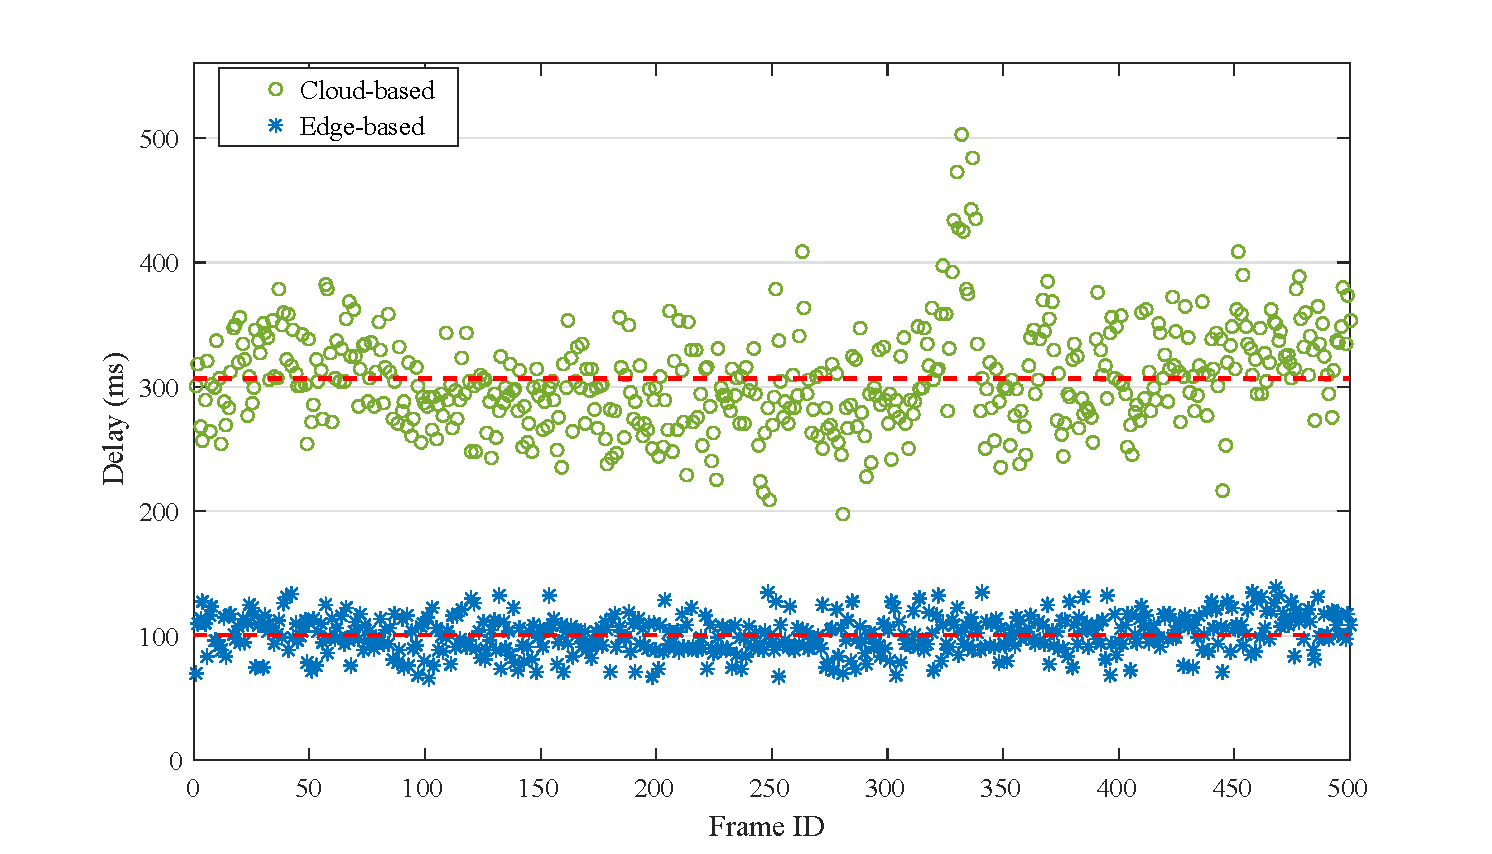
\includegraphics[width=1\columnwidth]{Fig2-4-v2v-delay.pdf}
  \bicaption{视频帧的传输延迟}{Transmission delay of video frames}
  \label{fig 2-4}
\end{figure}

本章为了比较基于边缘和基于云的服务的性能,实现了一个基于云的服务,将V1的实时视图通过基于LTE的通信传输到SDN控制器,然后通过LTE将视频发布给V2和V3。
其中500个视频帧被提取出来,平均大小为34.19 KB,范围从28.57 KB到42.41 KB。
通过图\ref{fig 2-4}的比较可以看出,基于边缘的服务在视频传输的性能方面表现更佳。
具体来说,V2和V3通过基于边缘的服务的平均传输延迟分别为100.8 ms和99.7 ms,而通过基于云服务的平均传输延迟分别为306.73 ms和308.93 ms。
此外,需要注意的是,在基于边缘的服务中,视频帧是通过 DSRC 广播给车辆V2和V3的,而基于LTE的通信在此应用中只支持单播。
因此,基于边缘的服务在资源利用方面具有很大的潜力,可以提高带宽效率并增强系统的可扩展性。
通过这个实验结果,可以验证本章提出的系统架构和基于边缘的服务在车联网中的实际可用性,并为未来的相关研究提供了有价值的参考。

\subsection{碰撞预警服务}

\begin{figure}[h] 
	\centering
	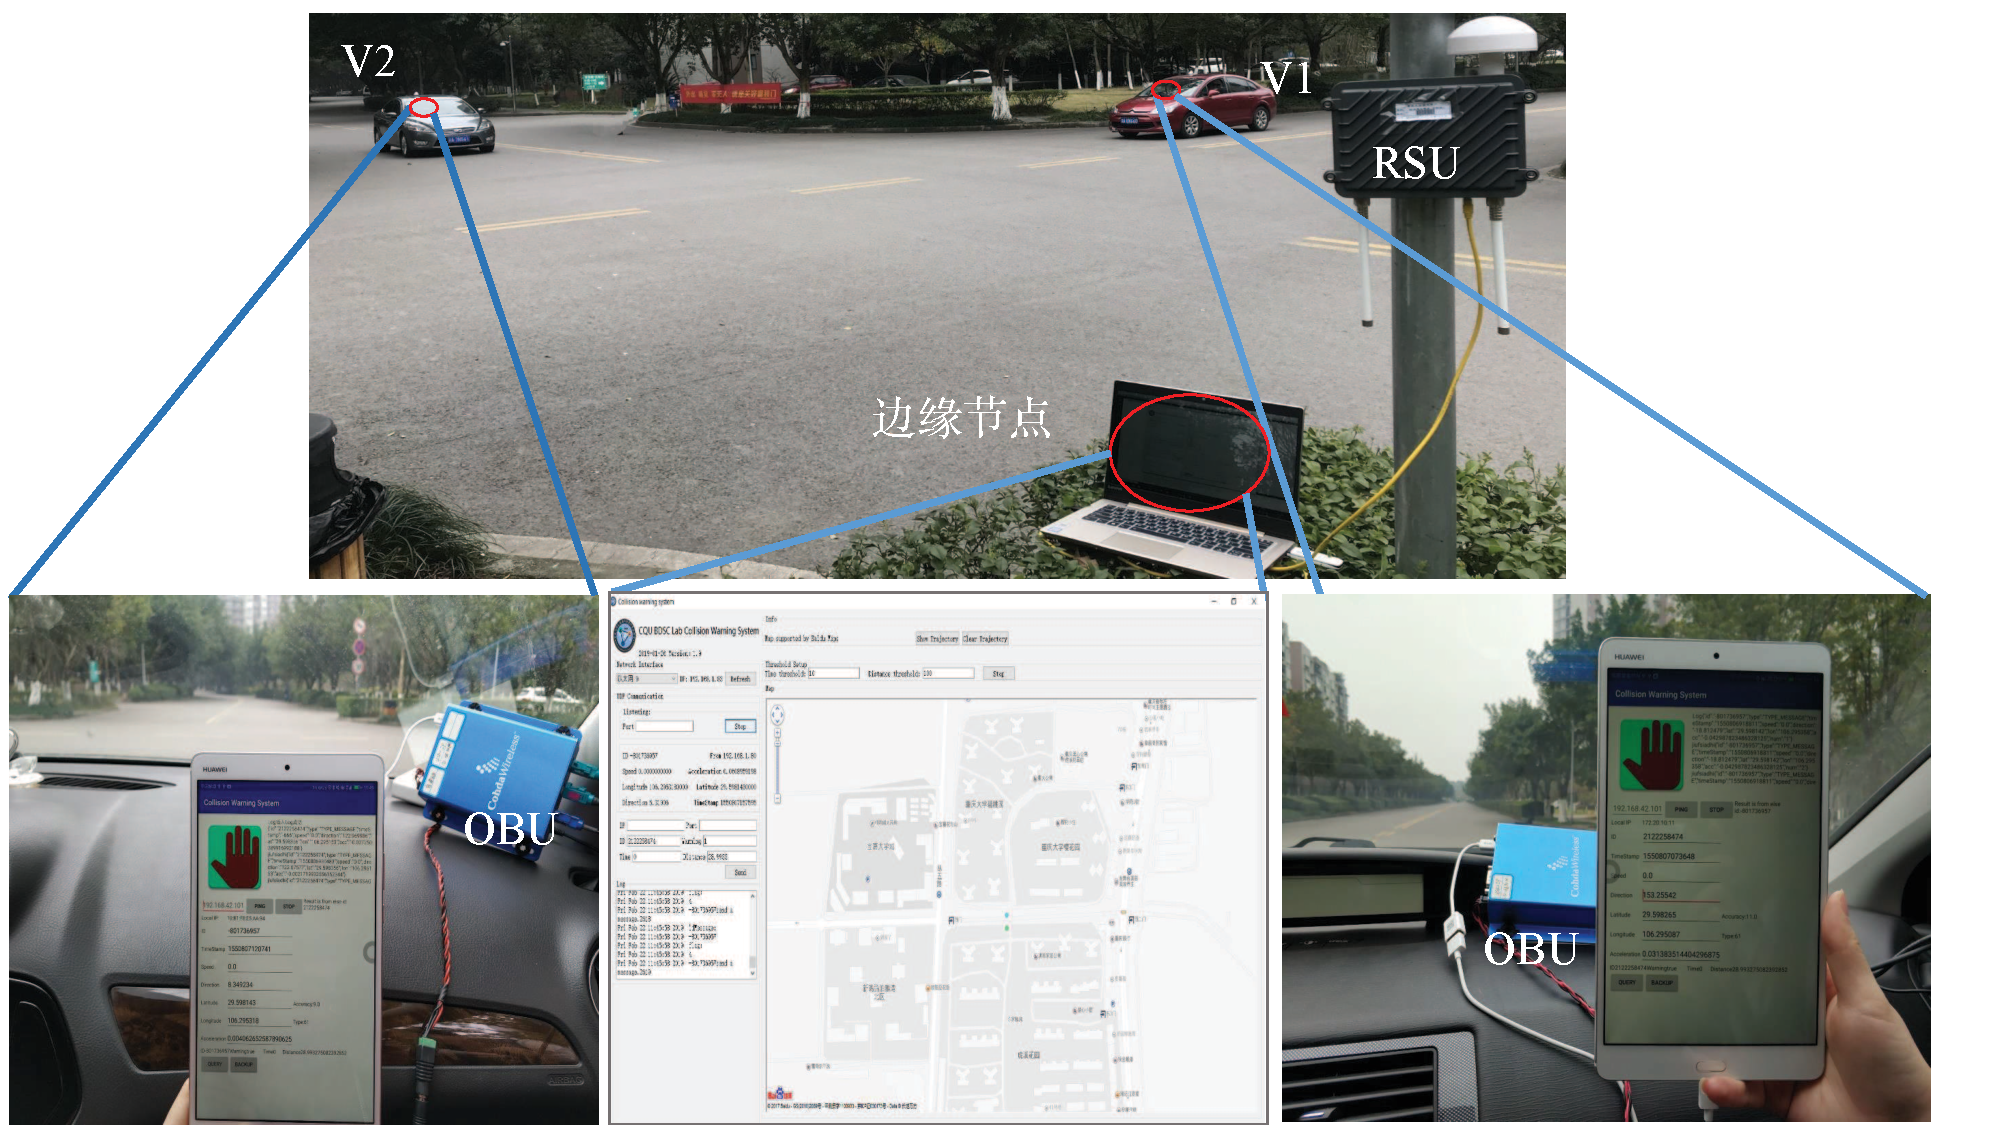
\includegraphics[width=1\columnwidth]{Fig2-5-case2.pdf}
	\bicaption{基于V2I通信的车辆碰撞预警}{Collision warning via V2I communications}
	\label{fig 2-5}
\end{figure}

碰撞预警服务旨在在两车之间有可能发生碰撞时触发警告信息,从而提高车辆的安全性。
在本系统中,云服务器配备2.5 GHz的CPU和2G的内存,而SDN控制器则可以通过基于LTE的通信与车辆进行通信。
为了支持大规模和实时的碰撞预警服务,计算和通信的工作量被卸载到实现服务功能的边缘服务器上。
如图\ref{fig 2-5}所示,本章考虑的场景是在道路交叉口部署一个RSU,一台笔记本与RSU连接,作为边缘服务器,并配备1.6GHz CPU和8G内存。
在该场景中,两辆汽车(即V1和V2)正在向十字路口移动,并相互靠近。
每辆车都配备了一个OBU,其与一个基于Android的平板电脑相连。
本章开发了一个基于Android系统的应用程序,用于收集车辆的实时状态,包括GPS坐标、速度、加速度、方向和时间戳等。
对于基于边缘的服务,车辆通过 DSRC 通信向边缘节点更新其状态。
根据从不同车辆收到的信息,边缘节点执行碰撞检测服务程序。
一旦检测有碰撞的风险,预警信息就会被触发,并通过 I2V 通信传送给相应的车辆。
然后,车辆中搭载的平板电脑上会显示一个停车标志,并伴随着振动和警告音。

\begin{figure}[h]
\centering
  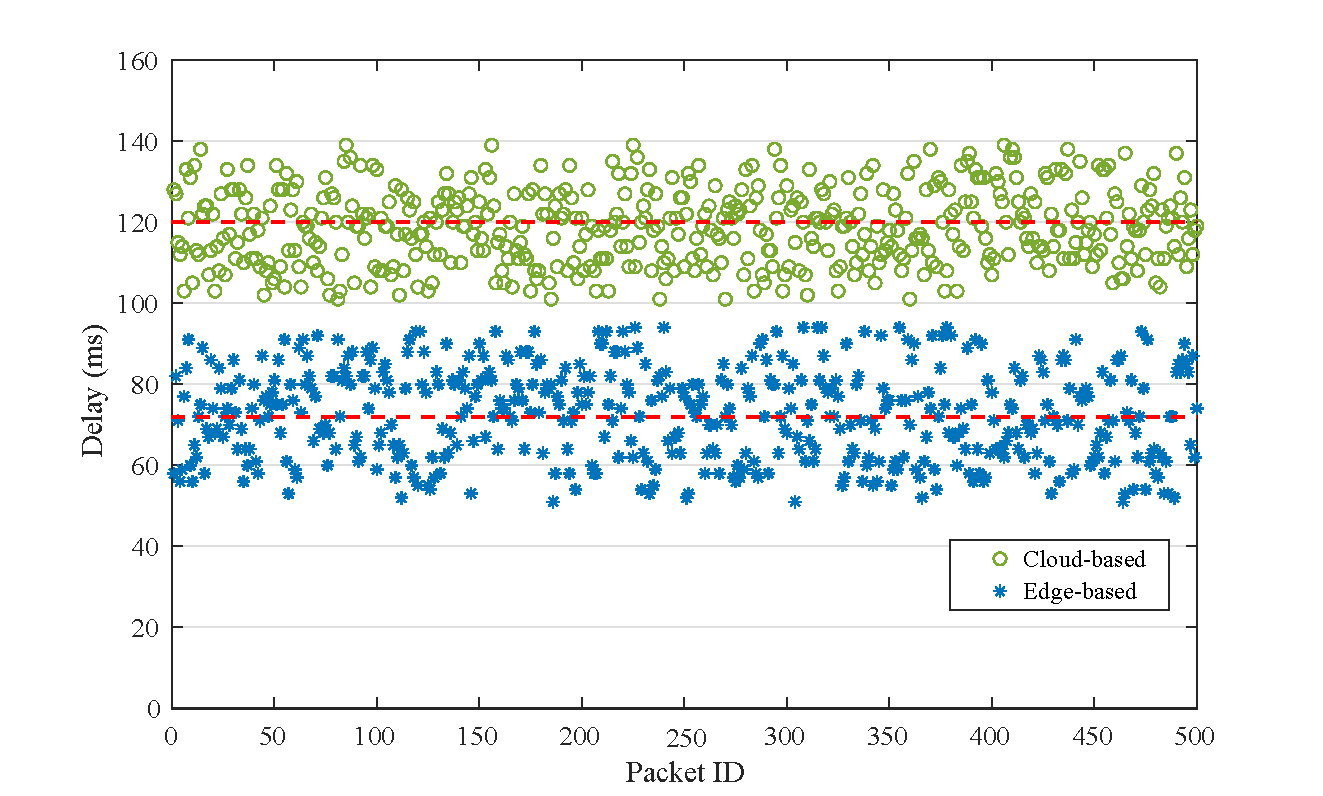
\includegraphics[width=1\columnwidth]{Fig2-6-v2i-delay.pdf}
  \bicaption{数据包的传输延迟}{Transmission delay of data packets}
  \label{fig 2-6}
\end{figure}

同时,本章还实现了基于云的服务,车辆通过LTE通信向云服务器更新它们的状态,而碰撞预警程序则在SDN控制器中实现。
一旦检测到潜在的碰撞,警告信息将通过 LTE 通信从云服务器传输到车辆。
为了比较基于边缘和基于云的服务的性能,图\ref{fig 2-6}比较了V1通过边缘和云服务的数据包延迟。
如前所述,边缘节点能够以更短的延迟接收来自车辆的更新,这对于如碰撞预警这类的安全相关的服务是至关重要的。
具体来说,车辆V1和V2通过基于边缘的服务的平均延迟分别为72.01 ms和74.03 ms,而V1和V2通过基于云的服务的平均延迟分别为120.08 ms和104.97 ms。
实验结果验证本章提出的基于边缘的服务的可行性,并为未来的相关研究提供了有价值的参考。

\subsection{启示}

本章提供的两个案例研究结果证明了基于边缘的服务在减少服务延迟方面的优越性,并且对未来ITS的实施提供了启示。
尽管作为迈向新的车联网范式的早期阶段,以及由于资源和环境的限制,上述案例研究只在小规模的环境中实施和评估了部分架构特征,但这些结果仍然有助于指导未来的研究和实践。

案例研究的结果表明,在一些相对理想的情况下,如低密度(2$\sim$3辆)、慢速(约25公里/小时),以及V2I(约20$\sim$50米)和V2V(约3$\sim$10米)通信距离较短情况下,DSRC的应用有效载荷数据率远低于其在PHY层的理论速率。
例如,“透视”服务中V2V通信的平均数据速率约为2.72 Mbps(34KB/100ms),这比DSRC声称的3$\sim$27 Mbps的速率要低得多。
因此,即使有基于边缘的服务,仍然需要 5G 等新兴技术来实现车联网中的超低延迟和安全关键应用,其是未来ITS需要重点关注的问题之一。

在未来的研究中,需要进一步评估基于NFV和NS的自适应资源分配和面向QoS的服务,以及基于服务卸载实现大规模和分布式服务的优势。
上述研究将进一步推动车联网领域的发展,并为相关应用场景提供更好的解决方案。
此外,还需要关注如何更好地处理车联网中的安全和隐私问题,以及如何将新兴技术与现有技术结合使用,以实现更加智能化和高效的应用场景。
例如,考虑与其他领域的交叉研究,如区块链、人工智能等,以实现更广泛的例如智慧城市、智能交通等应用场景。
综上所述,本章提供的案例研究为未来下一代ITS的发展和实现提供了有益的参考和指导。

\section{本章小结}\label{section 2-5}

本章为未来车联网的大规模、实时和可靠的信息服务提出了一个包括应用层、路由层、MAC层和物理层的分层服务架构。
所提新架构通过解耦控制和数据平面来实现逻辑上的集中控制。
在控制平面,SDN控制器与云服务器交互,管理车辆和边缘服务器的资源,并执行服务的自适应分配。
在数据平面,基于边缘的服务实现了资源和计算的卸载,以提高系统的可扩展性和性能。
此外,通过抽象和虚拟化异构资源来促进NFV和NS,这使得服务能够以高度灵活和可编程的方式实现。
同时,在新模式下出现了诸多挑战和机会。
例如,控制层的全局知识获取、虚拟层的异构资源管理、数据层的大规模数据传输等问题需要解决。
进一步,本章提出了一个跨层协议栈用于实现服务发现、分配和管理等功能。
此外,本章在现实世界的车联网环境中实现了系统原型,并提出了两个案例研究,其证明了所提架构的巨大潜力。
案例研究包括“透视”服务和碰撞预警服务,其实验结果表明,基于边缘的服务在减少服务延迟方面比基于云的服务更加优越,同时也提高了系统的可扩展性和性能。
然而,所提架构仍然需要 5G 等新兴技术的支持,以实现车联网中超低延迟和安全关键应用。
综上,本章提出的新架构为未来车联网提供了一个可行的解决方案,使车联网系统能够更加灵活、可靠和可扩展。